\documentclass[10pt,a4paper]{article}

\usepackage{amsmath}

\usepackage{inputenc}
\usepackage{fvextra}

\usepackage{algpseudocode}
\usepackage{algorithmicx}
\usepackage{amsfonts}
\usepackage{amssymb}
\usepackage{amsthm}
\usepackage[spanish]{babel}
\usepackage{bm}
\usepackage{booktabs} % To thicken table lines
\usepackage{bussproofs}
\usepackage{caption}
\usepackage{csquotes}
\usepackage{colortbl}
\usepackage{dsfont}
\usepackage{environ}
\usepackage[shortlabels]{enumitem}
\usepackage{fancyhdr}
\usepackage{forest}
\usepackage{geometry}
\usepackage{graphicx}
\usepackage[hidelinks]{hyperref}
\usepackage{ifthen}
\usepackage{multicol}
\usepackage{multirow}
\usepackage{sidecap}
\usepackage{stmaryrd}
\usepackage{tabularx}
\usepackage{titling}
\usepackage{tikz}
\usepackage{xcolor}
\usepackage{wrapfig}
\usepackage{minted}

\usetikzlibrary{arrows}
\usetikzlibrary{arrows.meta}
\usetikzlibrary{automata}
\usetikzlibrary{calc}
\usetikzlibrary{fit}
\usetikzlibrary{matrix}
\usetikzlibrary{positioning}
\usetikzlibrary{shapes.geometric}
\usetikzlibrary{shapes.multipart}

\newcommand{\red}[1]{{\color{red}#1}}
\newcommand{\green}[1]{{\color{green}#1}}
\newcommand{\blue}[1]{{\color{blue}#1}}
\newcommand{\violet}[1]{{\color{violet}#1}}
\newcommand{\orange}[1]{{\color{orange}#1}}

\newcommand{\nat}{\mathbb{N}}
\newcommand{\reales}{\mathbb{R}}

\newtheorem{theorem}{Teorema}
\newtheorem{coro}{Corolario}
\newtheorem{proposicion}{Proposición}
\newtheorem{lema}{Lema}


\usetikzlibrary{shapes.multipart}

\tikzstyle{demoBox} = [
draw=blue!20, very thick,
rectangle split, rectangle split parts=2, rounded corners, inner xsep=0.5cm,
rectangle split part fill = {blue!20, blue!5}
]

\tikzstyle{demoPart} = [
draw=blue!20, very thick,
rounded corners, inner xsep=0.5cm,
fill = blue!5
]
%\newcommand{\qed}{\begin{flushright}
%		$\blacksquare$
%\end{flushright}}

\NewEnviron{demo}[1][]{%
	\begin{center}
		\begin{tikzpicture}
			\node [demoBox](box){%
				\textbf{\scriptsize
					DEMOSTRACIÓN #1}
				\nodepart{two}
				\begin{minipage}{0.75\textwidth}
					\vspace*{0.1cm}
					\BODY
				\end{minipage}
			};
		\end{tikzpicture}
	\end{center}
}

\NewEnviron{demoPart}[1][]{%
	\begin{center}
		\begin{tikzpicture}
			\node [demoPart](box){%
				\begin{minipage}{0.75\textwidth}
					\vspace*{0.1cm}
					\BODY
				\end{minipage}
			};
		\end{tikzpicture}
	\end{center}
}


\title{Sistemas Operativos - Apuntes para final}
\author{Gianfranco Zamboni}

\usemintedstyle[cpp]{bordeland, tabsize=2}
%%%% CONFIGURACIONES %%%%

%% La coma de los reales es un punto
\decimalpoint{}

%%% Tamaño de pagina
%\geometry{
%	includeheadfoot,
%	left=2.54cm,
%	bottom=1cm,
%	top=1cm,
%	right=2.54cm
%}

%\stul{0.1cm}{0.2ex}

%% HEADER Y FOOTER
\pagestyle{fancy}

\fancyhf{}

\fancyhead[LO]{\rightmark} % \thesection\ 
\fancyhead[RO]{\small{\thetitle}}
\fancyfoot[CO]{\thepage}
\renewcommand{\headrulewidth}{0.5pt}
\renewcommand{\footrulewidth}{0.5pt}
\setlength{\headsep}{1cm}
\setlength{\headheight}{13.07225pt}

\renewcommand{\baselinestretch}{1.2}  % line spacing

%% Links en indice 
\hypersetup{
	linktoc=all,     %set to all if you want both sections and subsections linked
	linkcolor=blue,  %choose some color if you want links to stand out
}
\setcounter{tocdepth}{2}
\begin{document}

	\maketitle
	\tableofcontents

\newpage
\section{Introducción a la teoría de la información}
\subsection{La semilla del internet }

El telégrafo fue el antecesor del teléfono, un primer acercamiento a la comunicación de
mensajes vía una codificación. Desde fines de siglo XIX hasta segunda mitad del siglo XX,
aparecen las centrales de \textbf{conmutación de circuitos} (centrales telefónicas). A estas centrales
llegaban señales (cables) correspondientes a todas las casas que participacen en el sistema de
teléfonos. Las operadoras conectaban dos circuitos en sus tableros para cerrar el circuito y
permitir la comunicación entre las dos partes involucradas. Sin embargo, este tipo de comunicación tenía una gran falla: Si una central de conmutación de circuitos
dejaba de estar disponible por algún motivo de fuerza, todas las personas pertenecientes a esa
zona se verían incomunicadas.


A fines de los 50 se empieza a desarrollar la \textbf{conmutación de paquetes} buscando resolver este tema, es decir se busca una \textbf{red más tolerante a fallas}, \textbf{más flexible} a la hora de conectar dos puntos distantes y que \textbf{escale más facilmente} ante un incremento en el acceso a la comunicación.

La nueva red propuesta es una red descentralizada con mútiples caminos entre dos puntos que divide los paquetes en fragmentos que pueden llegar a destino a través de distintos caminos.

\subsection*{El modelo OSI}
En 1983 aparece una publicación de ISO para establecer un estándar que especifique la estructura de una arquitectura de red, que uniformice la forma de construir las redes de cominucación: el modelo OSI-ISO (Open Systems Interconnection).

\begin{figure}[h]
	\centering
	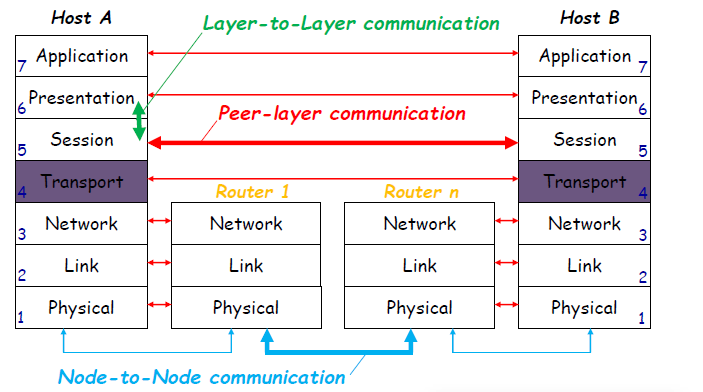
\includegraphics[width=0.65\textwidth
]{images/osi.png}
	\caption[Modelo OSI de Referencia]{Modelo OSI}
	\label{fig:osi}
\end{figure}

Este modelo está dividido en 7 capas, cada una de las cuales tiene una función definida que permitirán la comunicación coherente entre dos sistemas remotos.  

\begin{enumerate}
  \item La capa \textbf{física (Physical)} se encarga de enviar raw bits a través de los medios físicos disponibles en la red. 
  \item La capa de \textbf{enlace (Link)} se encarga de detectar errores en la transmisión y corregirlos, si es posible.
  \item La capa de \textbf{red (Network)} se encarga de resolver problemas de congestión dentro de la red, que paquetes se aceptan y la ruta que deben tomar los paquetes que se envían por la misma.
  \item La capa de \textbf{transporte (Transport)} se encarga de tomar la información provista por la capa de arriba, pasarla a la capa de red separada en pedazos más chicos (\textbf{chunks}) y se asegura que todas las partes lleguen a destino correctamente. 
  
  Esta es la primer capa \textbf{end-to-end}, es decir que entabla una "conversación" entre la máquina emisora (\textbf{Source}) y la destinataria (\textbf{Destination}). Las capas anteriores, usan protocolos de comunicación nodo a nodo, es decir, entre una máquina y su vecino inmediato y no entre el source y el destination que podrían estar separados entre sí por varios nodos.
  
  \item La capa de \textbf{sesión  (Session)} permite establecer sesiones entre dos máquinas distintas. Estas sesiones permiten sincronizar el pasaje de información entre ambas máquinas, deciden de quien es el turno para enviar información y evitar que ambas máquinas realizen operaciones críticas de manera simultanea.
  \item La capa de \textbf{presentación (Presentation)} procesa la información recibida, la estructura y la codifica de la manera necesaria para que pueda ser usada por la máquina.
  \item La capa de \textbf{aplicaciones (Application)} contiene los protocolos necesarios para que los usuarios puedan ver y leer la información.
\end{enumerate}

Además de estas funcionalidades, cada capa ofrece una interfaz que le permite comunicarse con las capas vecinas para hacer el pasaje de los datos entre ellas.

\subsection{Modelo TCP/IP}
\begin{figure}[H]
	\centering
	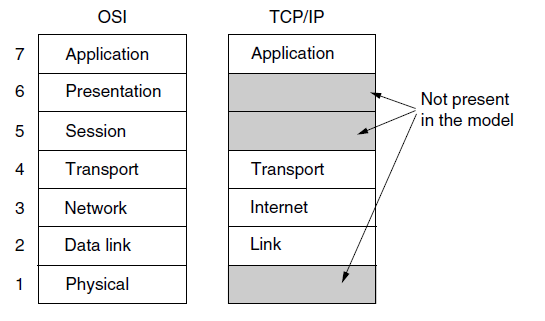
\includegraphics[width=0.65\textwidth
]{images/tcpip.png}
	\caption[Modelo TCP/IP de Referencia]{Modelo TCP/IP}
	\label{fig:tcp}
\end{figure}
\section{Nivel físico}
\red{
Concepto de Información. Fuentes de Información de Memoria Nula. Entropía. Longitud de un Código. Relación entre la entropía de una fuente de Información y la Longitud Media del código propuesto. Codificación de Huffman. Ancho de banda. Medios de transmisión guiados y no guiados. Punto a Punto y Compartidos (Broadcast). Modems. Modulación: Fase, Frecuencia, Amplitud y QAM. Conversión Analógico/Digital. Capacidad de Canal. Latencia. Producto delay-ancho de banda.

Unidad 2:
Nivel de Enlace: Punto a Punto. Servicios. Entramado. Manejo del enlace. Control de flujo. Control de errores: detección y corrección. Distancia de Hamming. Protocolo Stop \& Wait. Protocolos de ventana deslizante. Comparación de protocolos. Medidas de eficiencia.

Unidad 3:
Medios compartidos: Compartidos. Redes locales (LANs). Generalidades. Medios de transmisión. Nivel físico. Nivel de enlace de datos. Subcapa LLC (Logical Link Control): IEEE802.2. Subcapa MAC (Medium Access Control): IEEE 802.3 (Ethernet). CSMA/CD. Redes Inalámbricas. Frecuencia dedicada versus expandida (Spread Spectrum). WLANs. CSMA/CA. Wi-Fi: IEEE 802.11b/g/n. Repetidores. Puentes. LAN Switches. Conceptos de VLAN y troncales de VLANs (IEEE 802.1Q). Spanning Tree Protocol.

Unidad 4:
Nivel de red. Conmutación y Forwarding. Subredes. Implementación: circuitos virtuales y datagramas. Control de flujo. Concepto de Ruteo. Protocolo IP. Direccionamiento. Broadcasting. Ejemplos de subnetting. Protocolo ARP. Forwarding. ICMP. Traducción de direcciones (NAT).

Unidad 5:
Ruteo Externo e Interno. Distance Vector y Link State. Los protocolos RIP y OSPF. Áreas. Inundación confiable.

Unidad 6:
Nivel de transporte. Servicios. Primitivas. Protocolos. Servidores de nombres. Manejo de conexión: establecimiento, uso y liberación. Manejo de conexión basados en tiempo. Direccionamiento. Control de flujo. Asignación de buffers. Recuperación de caídas. Multiplexado. Protocolos de nivel 4: Transport Control Protocol (TCP). User Datagram Protocol (UDP) . Mecanismos de control de congestión. Cálculo del RTO. Control de Flujo. Control de errores. Determinación de la performance.

Unidad 7:
Introducción al problema de congestión. Curvas de Trafico Enviado vs entregado. Resultado con buffer infinito. Causas de congestión. Control de flujo vs Control de congestión. Taxonomia de Yang y Redan. Soluciones de lazo cerrado y abierto. Concepto de sistemas realimentados. Métricas a sensar para las realimentación. Realimentación implícita y explicita. Determinación de la performance.

Unidad 8:
Aplicaciones. Correo Electrónico. Protocolos : SMTP, POP3 e IMAP, MIME. Servidores World Wide Web. HTTP. Servidor de Nombres: DNS. Jerarquía de dominios. Resolución de nombres.

Unidad 9:
Seguridad en Redes. Marco de Trabajo. Criptografía. Seguridad. Privacidad. Protocolos de Clave Pública y Privada. Algoritmos: DES, 3DES, AES, RSA, MD5 y SHA .Ventajas y desventajas de cada uno. Sus aplicaciones (Autorización, Firma, Confidencialidad e Integridad). Distribución de Claves Públicas. Firewalls. Tunneling. Conceptos de amenazas, ataques, intrusiones.
}
\end{document}

